% =====================================================================
%  Chapitre 3 -- LSTM et GRU : dompter la memoire
%  Partie a : la cellule LSTM, ses portes, le convoyeur
% =====================================================================
\section{Chapitre 3 --- LSTM et GRU}

\chapterslide{Chapitre 3}{LSTM et GRU : dompter la mémoire}%
{5 h --- portes, état de cellule, survie du gradient, variantes}%
{\textbf{Objectifs.} Nommer et expliquer les trois portes du LSTM ; comprendre
pourquoi l'état de cellule laisse passer le gradient ; comparer LSTM et GRU ;
situer le bidirectionnel et l'empilement.}

\begin{frame}{Le diagnostic du chapitre 2}
\begin{columns}[t]
\begin{column}{0.48\textwidth}
\begin{wbox}[Le RNN simple oublie]
Sa mémoire est réécrite à \textbf{chaque pas} : $h_t = \tanh(\ldots)$ écrase
$h_{t-1}$ entièrement. Après quelques dizaines de pas, le début de la séquence
a disparu.
\end{wbox}
\begin{wbox}[Et le gradient avec]
Le produit des dérivées s'effondre : le réseau ne peut pas apprendre une
dépendance à 30 pas de distance.
\end{wbox}
\end{column}
\begin{column}{0.48\textwidth}
\begin{kbox}[L'intuition de la solution]
Et si, au lieu de tout réécrire, on ajoutait un \textbf{chemin protégé} qui
transporte l'information, avec des \textbf{portes} qui décident quoi garder,
quoi écrire, quoi dévoiler ?
\end{kbox}
\begin{solbox}[C'est exactement le LSTM (1997)]
Hochreiter et Schmidhuber : \textbf{Long Short-Term Memory}. La idée tient en
un mot : un \emph{convoyeur}.
\end{solbox}
\end{column}
\end{columns}
\end{frame}

\begin{frame}{La cellule LSTM, en un coup d'œil}
\begin{center}
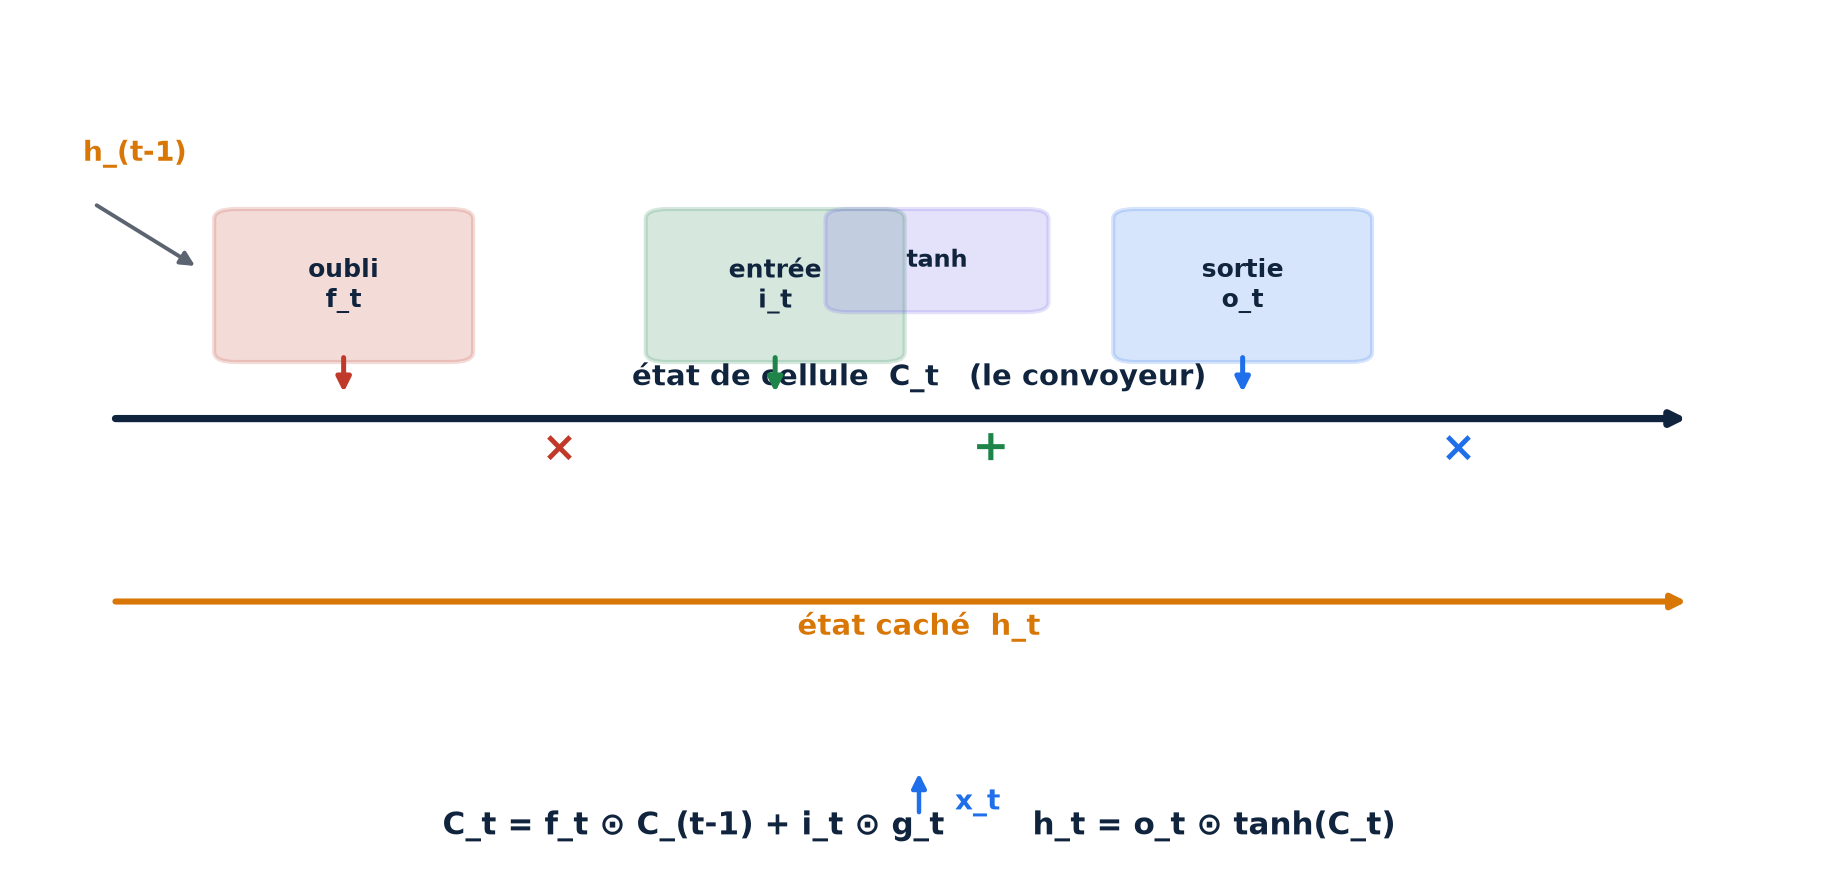
\includegraphics[width=0.95\textwidth]{t01_lstm_cellule.png}
\end{center}
\end{frame}

\begin{frame}{Les trois portes, une par une}
\begin{columns}[t]
\begin{column}{0.32\textwidth}
\begin{wbox}[Porte d'oubli $f_t$]
Vaut entre 0 et 1 à chaque pas : 0 = jeter, 1 = garder.

« Quand un nouveau sujet commence, oublie l'ancien. »
\end{wbox}
\end{column}
\begin{column}{0.32\textwidth}
\begin{wbox}[Porte d'entrée $i_t$]
Combien de la \textbf{nouvelle} information écrire dans l'état.

« Ce mot compte : range-le. »
\end{wbox}
\end{column}
\begin{column}{0.32\textwidth}
\begin{wbox}[Porte de sortie $o_t$]
Combien de l'état \textbf{révéler} à la sortie.

« Garde-le en mémoire, mais ne le montre pas encore. »
\end{wbox}
\end{column}
\end{columns}
\vspace{2mm}
\begin{kbox}[Toutes les portes sont apprises]
Chaque porte est une couche sigmoïde sur $[x_t, h_{t-1}]$ : le réseau apprend
\emph{quand} ouvrir et fermer. Ce n'est pas de la logique codée à la main.
\end{kbox}
\end{frame}

\begin{frame}{Les équations, commentées}
\begin{center}
\small
\begin{tabular}{@{}lll@{}}
\toprule
\textbf{Porte / état} & \textbf{Formule} & \textbf{Rôle} \\
\midrule
oubli & $f_t = \sigma(W_f[x_t, h_{t-1}] + b_f)$ & garder l'ancien \\
entrée & $i_t = \sigma(W_i[x_t, h_{t-1}] + b_i)$ & accepter le nouveau \\
candidat & $\tilde{C}_t = \tanh(W_C[x_t, h_{t-1}] + b_C)$ & ce qu'on proposerait \\
\textbf{état} & $C_t = f_t \odot C_{t-1} + i_t \odot \tilde{C}_t$ & \textbf{mise à jour} \\
sortie & $o_t = \sigma(W_o[x_t, h_{t-1}] + b_o)$ & combien montrer \\
sortie cachée & $h_t = o_t \odot \tanh(C_t)$ & ce que le réseau publie \\
\bottomrule
\end{tabular}
\end{center}
\vspace{1mm}
\begin{kbox}[La seule ligne à retenir]
$C_t = f_t \odot C_{t-1} + i_t \odot \tilde{C}_t$ : une \textbf{addition}
contrôlée --- pas un écrasement.
\end{kbox}
\end{frame}

\begin{frame}{Les portes en action}
\begin{center}
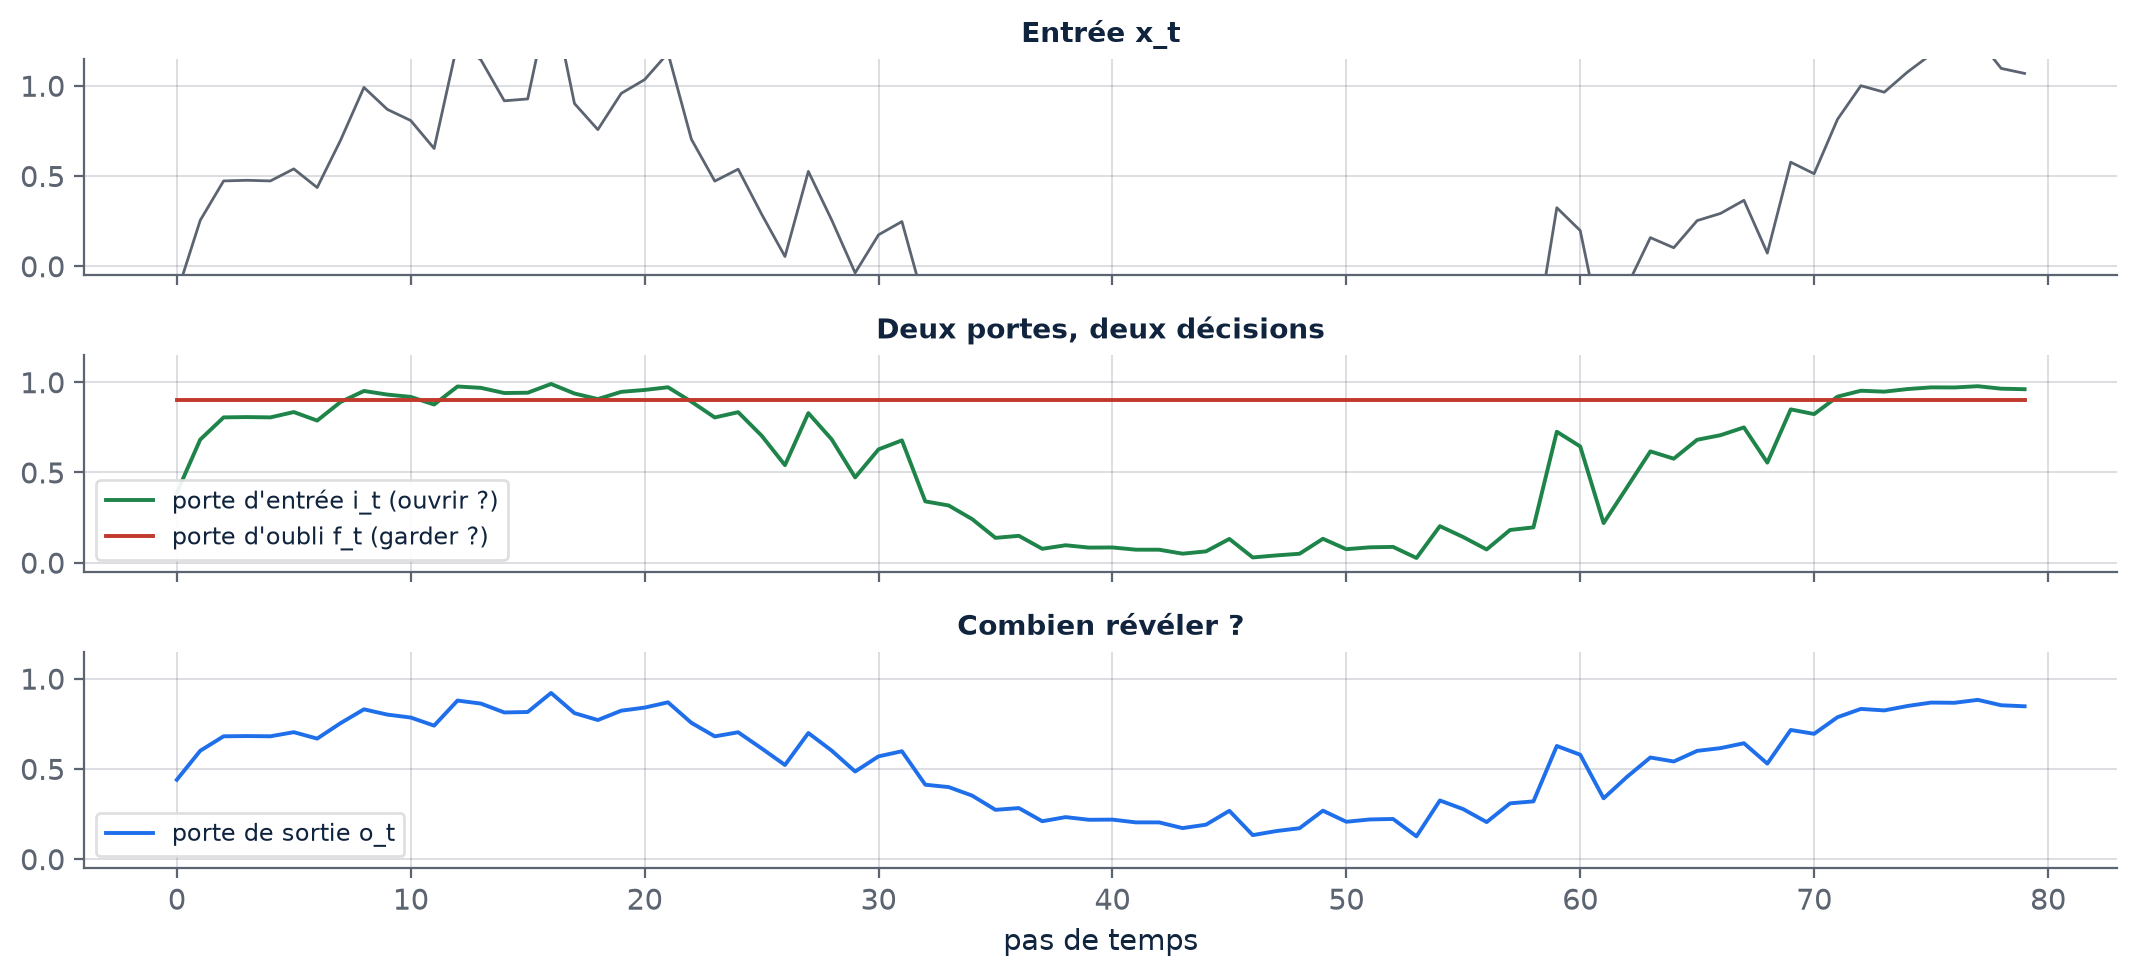
\includegraphics[width=0.88\textwidth]{t02_portes.png}
\end{center}
\vspace{1mm}
\begin{kbox}[Lecture]
Sur une entrée oscillante, la porte d'entrée suit l'activité, la porte d'oubli
reste ouverte, la porte de sortie module. Ces valeurs sont \textbf{calculées},
pas affichées à la main.
\end{kbox}
\end{frame}

\begin{frame}{Le convoyeur : pourquoi le gradient passe}
\begin{center}
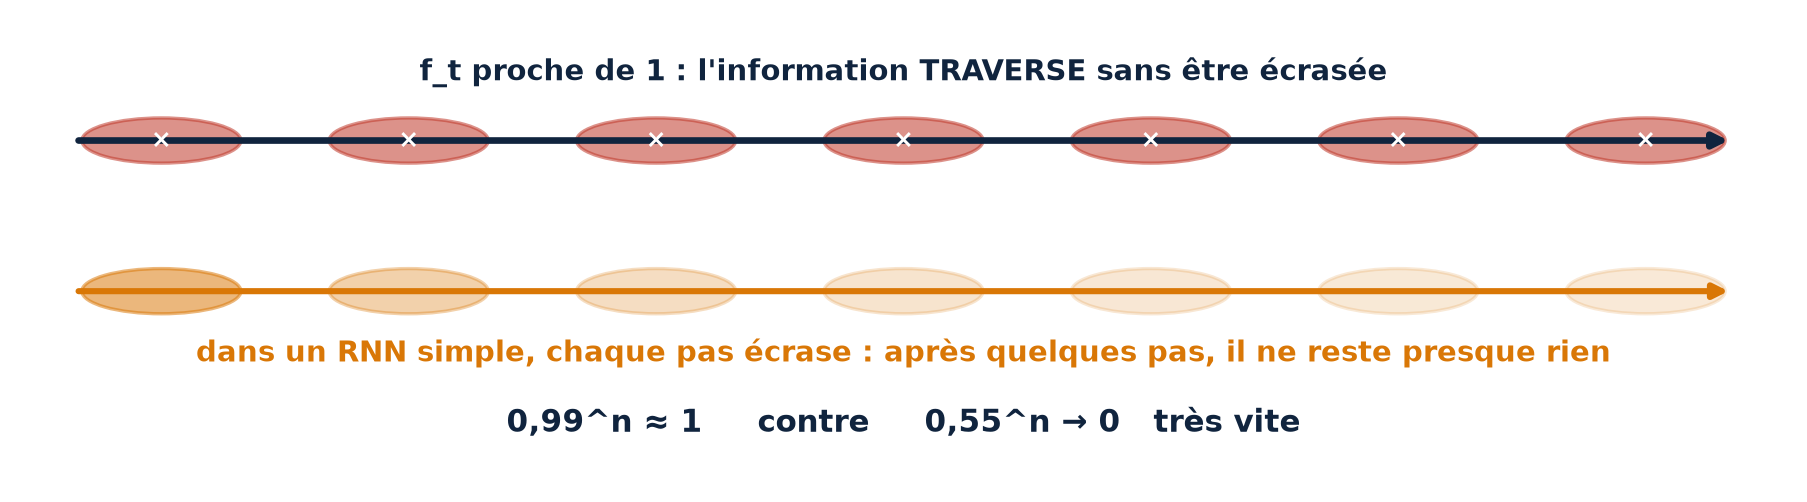
\includegraphics[width=0.92\textwidth]{t03_conveyor.png}
\end{center}
\vspace{1mm}
\begin{solbox}[Le calcul]
Le gradient de $C_t$ par rapport à $C_{t-1}$ vaut $f_t$ (plus les termes
additifs). Avec $f_t \approx 0{,}99$, il reste $0{,}99^{30} = 0{,}74$ du
gradient après 30 pas --- contre $0{,}55^{30} = 2 \times 10^{-8}$ dans un
RNN simple.
\end{solbox}
\end{frame}

\begin{frame}{Survie du gradient : le calcul}
\begin{columns}[t]
\begin{column}{0.96\textwidth}
\begin{itemize}
  \item RNN simple, $r = 0{,}55$ : à 30 pas, il reste $2 \times 10^{-8}$.
  \item LSTM, $f = 0{,}99$ : à 30 pas, il reste $0{,}74$.
  \item La \textbf{multiplication additive} de l'état change tout.
\end{itemize}
\begin{solbox}[C'est la thèse du chapitre]
Le LSTM ne « se souvient mieux » par magie : il offre un chemin de gradient
\emph{presque} non dégradé.
\end{solbox}
\end{column}
\end{columns}
% [fix] figure sortie
\end{frame}

\begin{frame}{Survie du gradient : le calcul --- la figure}\begin{center}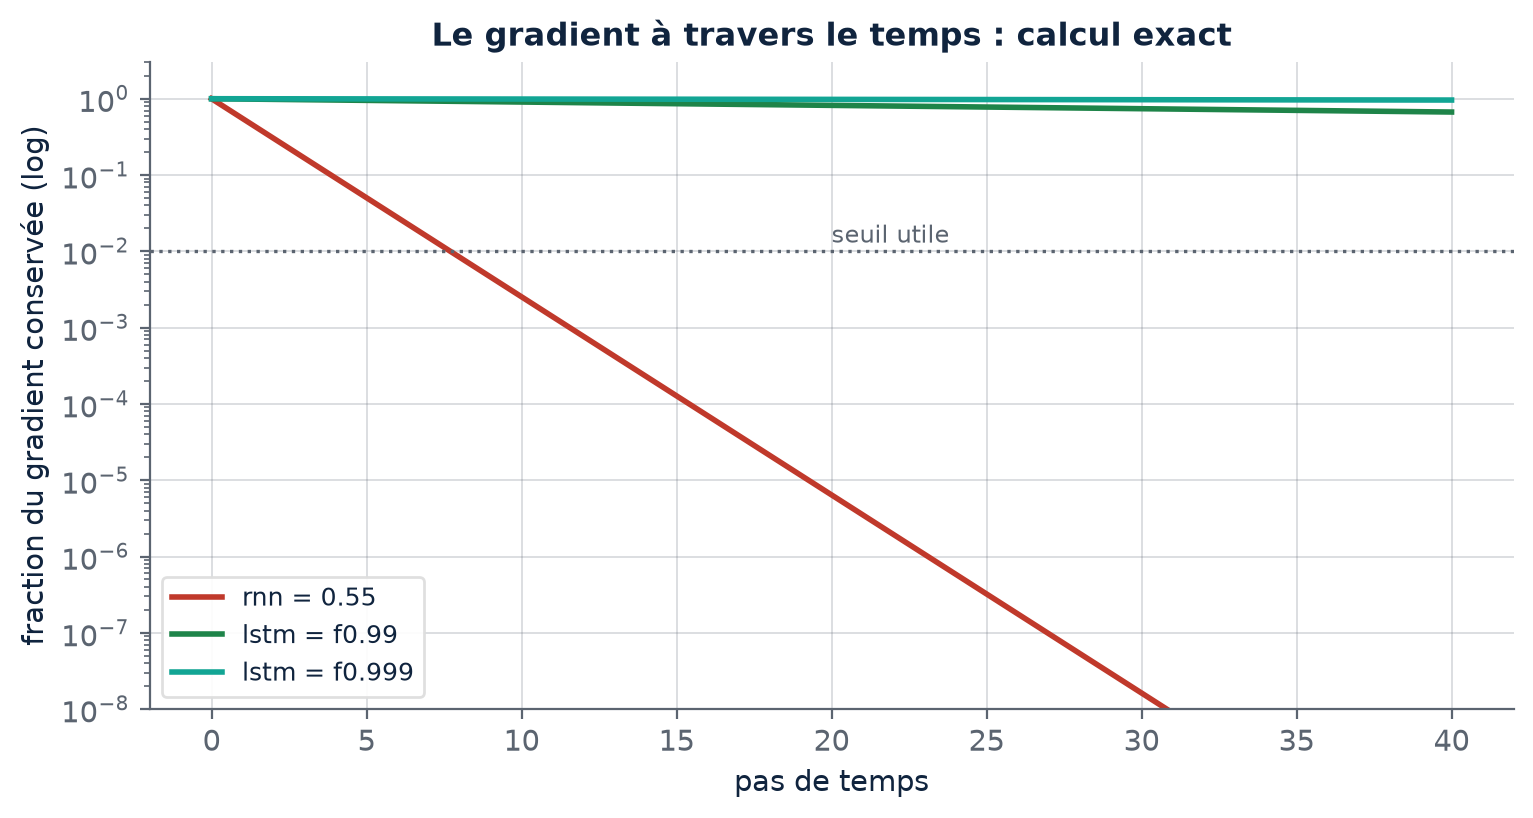
\includegraphics[width=.92\textwidth]{t04_survie_gradient.png}\end{center}\end{frame}

\begin{frame}{Quiz 3 --- LSTM}
\begin{qbox}[Question 1]
Combien de portes possède un LSTM, et quelles sont-elles ?
\begin{itemize}
  \item[(a)] 2 (entrée, sortie) \quad (b) 3 (oubli, entrée, sortie) \quad
  (c) 4 (dont reset)
\end{itemize}
\end{qbox}
\begin{qbox}[Question 2]
Quelle ligne met à jour l'état de cellule ?
\begin{itemize}
  \item[(a)] $h_t = o_t \odot \tanh(C_t)$ \quad (b) $C_t = f_t \odot C_{t-1} +
  i_t \odot \tilde{C}_t$ \quad (c) $f_t = \sigma(\ldots)$
\end{itemize}
\end{qbox}
\begin{qbox}[Question 3]
Avec $f_t = 0{,}99$ à chaque pas, le gradient après 30 pas vaut environ :
\begin{itemize}
  \item[(a)] $0{,}74$ \quad (b) $2 \times 10^{-8}$ \quad (c) $0$
\end{itemize}
\end{qbox}
\begin{solbox}[Réponses]
\textbf{1.} (b). \quad \textbf{2.} (b) : l'ajout contrôlé, pas l'écrasement. \quad
\textbf{3.} (a) : $0{,}99^{30} = 0{,}740$.
\end{solbox}
\end{frame}
